
\documentclass{vgtc}                          % final (conference style)
%\documentclass[review]{vgtc}                 % review
%\documentclass[widereview]{vgtc}             % wide-spaced review
%\documentclass[preprint]{vgtc}               % preprint
%\documentclass[electronic]{vgtc}             % electronic version

\usepackage{mathptmx}
\usepackage{graphicx}
\usepackage{times}

%% We encourage the use of mathptmx for consistent usage of times font
%% throughout the proceedings. However, if you encounter conflicts
%% with other math-related packages, you may want to disable it.

%% If you are submitting a paper to a conference for review with a double
%% blind reviewing process, please replace the value ``0'' below with your
%% OnlineID. Otherwise, you may safely leave it at ``0''.
\onlineid{0}

%% declare the category of your paper, only shown in review mode
\vgtccategory{Research}

%% allow for this line if you want the electronic option to work properly
\vgtcinsertpkg

%% In preprint mode you may define your own headline.
%\preprinttext{To appear in an IEEE VGTC sponsored conference.}

%% Paper title.

\title{Interactive Multiplots For Comparing Coverage Effectiveness}

%% Author and Affiliation (multiple authors with single affiliations).
%%\author{Roy G. Biv\thanks{e-mail: roy.g.biv@aol.com} %
%%\and Ed Grimley\thanks{e-mail:ed.grimley@aol.com} %
%%\and Martha Stewart\thanks{e-mail:martha.stewart@marthastewart.com}}
%%\affiliation{\scriptsize Martha Stewart Enterprises \\ Microsoft Research}

%% Author and Affiliation (multiple authors with multiple affiliations)
\author{Adam M. Smith\thanks{e-mail: ams292@cs.pitt.edu} %
\and Joshua J. Geiger\thanks{e-mail:jjg???@cs.pitt.edu}} %
\affiliation{\scriptsize University of Pittsburgh}


\abstract{Software testing increases confidence in the correctness of application source code.  Using different orderings of a test suite can enable the earlier detection of defects which allows developers to start fixing them sooner.  Finding the best ordering is difficult and there are many approaches that prioritize the ordering, resulting in many possible test suite orderings to choose from.  This paper presents a tool that allows the user to visually examine  the results of several test suite prioritization techniques and to use interaction to gain insights about the properties of the test suite and its different orders. }

%% ACM Computing Classification System (CCS). 
%% See <http://www.acm.org/class/1998/> for details.
%% The ``\CCScat'' command takes four arguments.

%%\CCScatlist{ 
 %% \CCScat{K.6.1}{Management of Computing and Information Systems}%
%%{Project and People Management}{Life Cycle};
%%  \CCScat{K.7.m}{The Computing Profession}{Miscellaneous}{Ethics}
%%}

%% Copyright space is enabled by default as required by guidelines.
%% It is disabled by the 'review' option or via the following command:
% \nocopyrightspace

%%%%%%%%%%%%%%%%%%%%%%%%%%%%%%%%%%%%%%%%%%%%%%%%%%%%%%%%%%%%%%%%
%%%%%%%%%%%%%%%%%%%%%% START OF THE PAPER %%%%%%%%%%%%%%%%%%%%%%
%%%%%%%%%%%%%%%%%%%%%%%%%%%%%%%%%%%%%%%%%%%%%%%%%%%%%%%%%%%%%%%%%

\begin{document}

%% The ``\maketitle'' command must be the first command after the
%% ``\begin{document}'' command. It prepares and prints the title block.

%% the only exception to this rule is the \firstsection command
\firstsection{Introduction}

\maketitle

%% \section{Introduction} 

Inevitably, errors are made while designing and implementing software systems. Software developers execute tests $\{t_1, t_2, t_3,\ldots, t_n\}$ in a test suite $T$ to isolate defects and gain confidence in the correctness of the code.  Each test case in the test suite exercises specific points in the system, comparing the actual output of the code to the hand computed expected one.  If a test fails, then a defect is present in the area that the test executes.  As the source code grows in size and number of features, new tests are written for the new functionality.  These new tests, however, do not obviate the old ones.  To ensure that the new features do not cause the system to regress, developers include every previously written test in the collection of tests.  This process of executing and re-executing the entire test suite is known as regression testing.  

Gradually, adding new tests and retaining old ones increases the size of the test suite until its execution time can become prohibitively expensive.  In some cases the regression test suite runs for several weeks \cite{empiricalfamily}.  One method of altering the test suite to resolve this issue is test suite prioritization \cite{rothermelprioritizing2001}.  Test suite prioritization attempts to find a reordering of the test cases that is more likely to locate defaults earlier in the execution of the test suite without risking the loss of coverage by removing a test.  The tests are ordered based on certain criteria that are obtained during a process called coverage monitoring.  

Coverage monitoring measures the code coverage of a test case $t_i$.  Code coverage describes any metric that enumerates specific points in the source code that are executed when a test is run, whether they are a line, a block, a method, a branch \cite{zhu}, or some other type. Each specific program point is called a requirement.  Given a test suite $T$, coverage monitoring gives a set of requirements $R(T) = \langle r_1, r_2,\ldots,r_m \rangle$.  Each individual test $t_i$ is associated with a subset of requirements $R(t_i) \subseteq R(T)$.  Each test is said to cover its associated set of requirements.  

\begin{figure}[t]
\centering
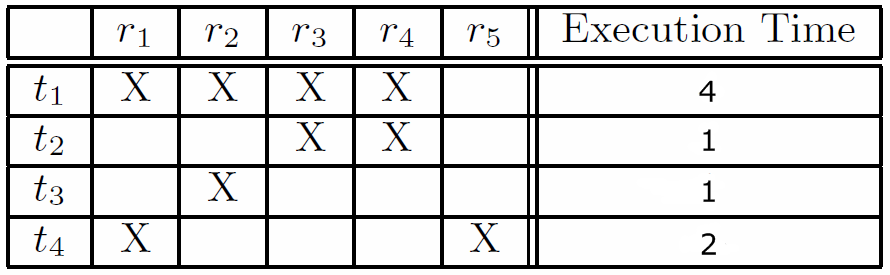
\includegraphics[scale=.2]{CoverageMatrix}
\caption{Example Test Suite}
\end{figure}
\label{fig:example}

\begin{figure}[ht]
\centering
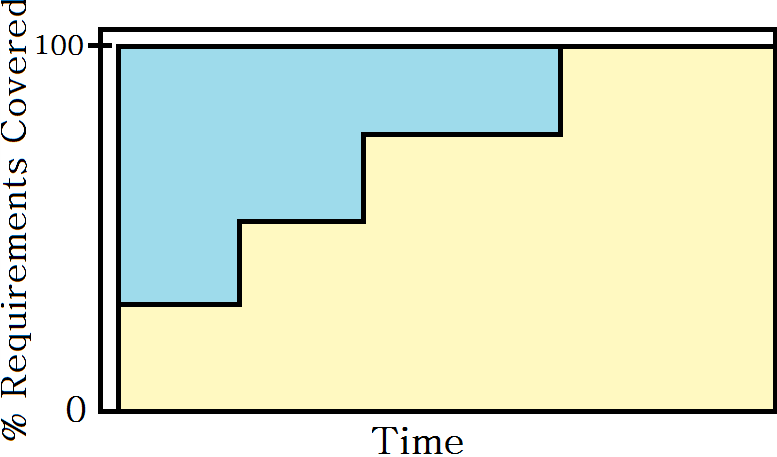
\includegraphics[scale=.2]{ce}
\caption{Coverage Effectiveness}
\end{figure}
\label{fig:ce}

Figure \ref{fig:example} shows an example of a test suite with 4 tests and 5 requirements.  An X in a cell represents that the test for that row covers the requirement in that column.  Imagine that the shown test suite is run in its original order.  In this case all of the requirements are not covered until 8 time units have passed.  Conversely, if the test suite is executed in reverse order all of the requirements are covered in 4 time units.  Covering all of the requirements sooner gives a better chance to find faults sooner so that the developers can begin to make changes at an earlier time.  

The metric coverage effectiveness \cite{ce} was developed in order to rate a test suite prioritization.  CE is derived from the step function of the cumulative coverage of a test suite as shown in Figure \ref{fig:ce}.  Each test suite offers the possibility of covering more total requirements.  So when the cumulative coverage is plotted against time a step function is formed.  CE itself is calculated by dividing the area under the step function for the actual order by the area under the curve of a test suite that covers all of its requirements instantly.  This value is between 0 and 1 where 0 means that no requirements were covered, and 1 means that all of the requirements were covered instantly.

\section{Motivation}

There are a total of $n$! possible orderings of a test suite where $n$ is the number of tests.  Clearly for most test suites these cannot all be enumerated to find ordering with the highest CE.  For this reason there are several algorithmic ways to find good orderings, including random sampling.  However, it is difficult to interpret the results of several algorithms or random samples by reading text alone.  Therefore, this project aimed to create a visualization that can allow software testers to instantly see how algorithmic prioritizers perform and also to examine a set of random random prioritizations simultaneously.  There is related work in the field of visuzaling test suites \cite{tarantula} \cite{bart}, however, they focus on fault localization or other features of a test suite.

\begin{figure}
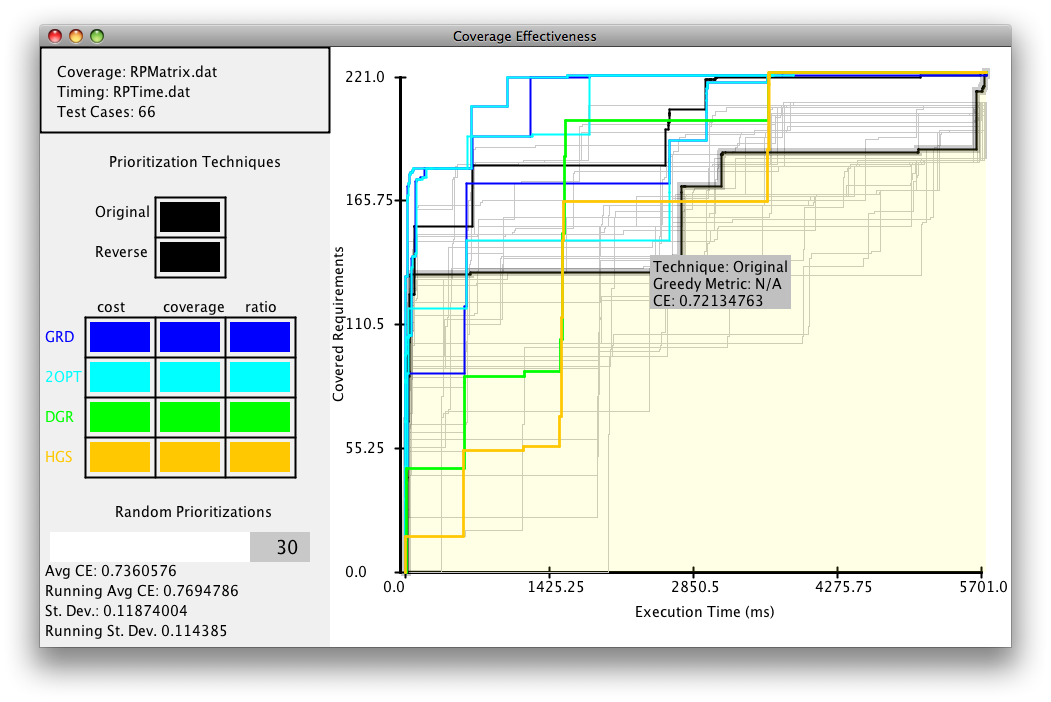
\includegraphics[scale=.3]{screenshot}
\end{figure}

%% if specified like this the section will be ommitted in review mode
\acknowledgements{
The authors wish to thank Gregory Kapfhammer, Manos Renieris, and Liz Marai for assistance with this project.}

\bibliographystyle{abbrv}
%%use following if all content of bibtex file should be shown
%\nocite{*}
\bibliography{myBibtexDB}
\end{document}
